\section{Decision Trees}
The space is recursively partitioned, each node in the tree is responsible for establishing a subdivision of the space, the final leaf corresponds to the output.
\begin{itemize}
    \item Each node corresponds to only one attribute
    \item Branching is determined by the value of the attribute
    \item Each leaf is associated with a class
\end{itemize}
For each training set it is possible to general a decision tree with a path to the correct leaf for each sample, the generated tree however does not generalize over other test examples (overfitting). It is therefore necessary to regularize to create more compact trees that can generalize.
\begin{center}
    \begin{tabular}{c c}
        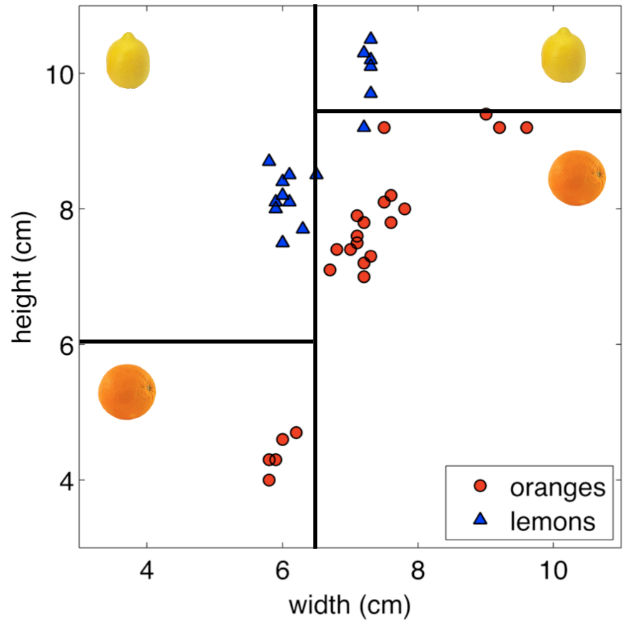
\includegraphics[width=0.45\textwidth]{images/DecisionTrees1.png} &
        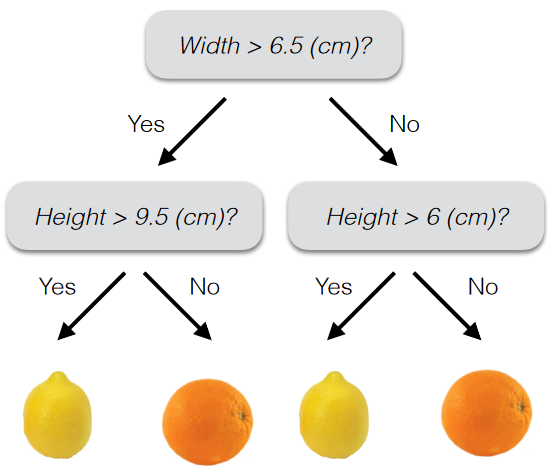
\includegraphics[width=0.5\textwidth]{images/DecisionTrees2.png}
    \end{tabular}
\end{center}

\subsection{Learning Decision Trees}
Creating the simplest decision tree is a complete NP problem, so heuristic solutions are used to simplify the problem:
\begin{enumerate}
    \item start with an empty decision tree
    \item divide the tree on the attribute that subdivides the examples among them in the best way
    \item recursively repeat the process
\end{enumerate}

\subsubsection{ID3 Algorithm}
ID3 is a popular for learning decision trees and works like this:
\begin{enumerate}
    \item creates a root node $r$
    \item if all examples $S$ belong to the same class $y$ returns the root node with label $y$
    \item if $A$ (attributes) is empty it will return $r$ with the same value as the most frequent class in $S$
    \item else select the optimal node:
    \begin{enumerate}
        \item[a.] partitions the set $S$ into subsets using the attribute for which entropy is minimized
        \item[b.] creates a decision node containing the selected attribute
        \item[c.] applies recursion in the underlying branch
    \end{enumerate}
\end{enumerate}

\newpage